\newpage
\section{Прочие настройки}

\subsection{Настройка фонового изображения и логотипа}

Настройка фонового изображения и логотипа возможна только при входе пользователя под ролью <<Администратор>>.

Настройка выполняется в меню \mm{Настройки \str Внешний вид} на вкладке \dm{Администратор} (Рисунок \ref{img_oth_vid}) (она становится доступна только под администратором).

\begin{figure}[ht]\centering
 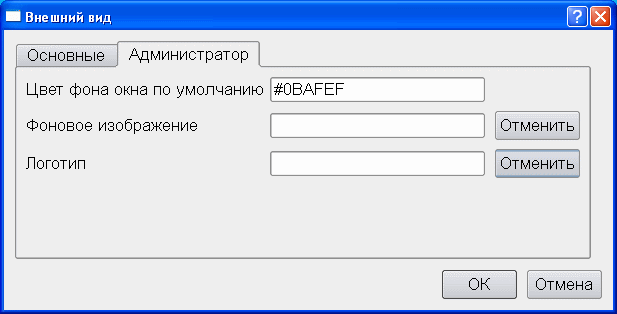
\includegraphics[width = 0.6\textwidth ,keepaspectratio]{oth_vid}
 \caption{Настройка внешнего вида}
 \label{img_oth_vid}
\end{figure}

Для изменения цвета фона окна следует щелкнуть левой кнопкой мыши по полю \dm{Цвет фона окна по умолчанию} и в открывшемся окне подобрать цвет и нажать кнопку \btn{OK}.

Для добавления фонового изображения в окно программы нужно щелкнуть левой кнопкой мыши в поле \dm{Фоновое изображение}, указать путь к файлу изображения и нажать кнопку  \btn{Открыть}. После чего файл будет загружен в БД. Размер загружаемого файла не должен превышать 250 Кб. Аналогичным образом загружается логотип в поле \dm{Логотип}. Рекомендуемый размер логотипа – не более 100х100 пискелей.

\subsection{Настройка соединений с внешними системами}

\tmis~может взаимодействовать с другими системами: 
\begin{itemize}
 \item Аппаратами функциональной диагностики в формате DICOM;
 \item Региональной системой автоматизации родовспоможения(РИСАР);
 \item Системами, установленными в МИАЦ региона. 
\end{itemize}

Для обеспечения взаимодействия необходимо выполнить настройки в меню \mm{Настройки \str Настройки \tmis} (Рисунок \ref{img_oth_dicomm}).

\begin{figure}[ht]\centering
 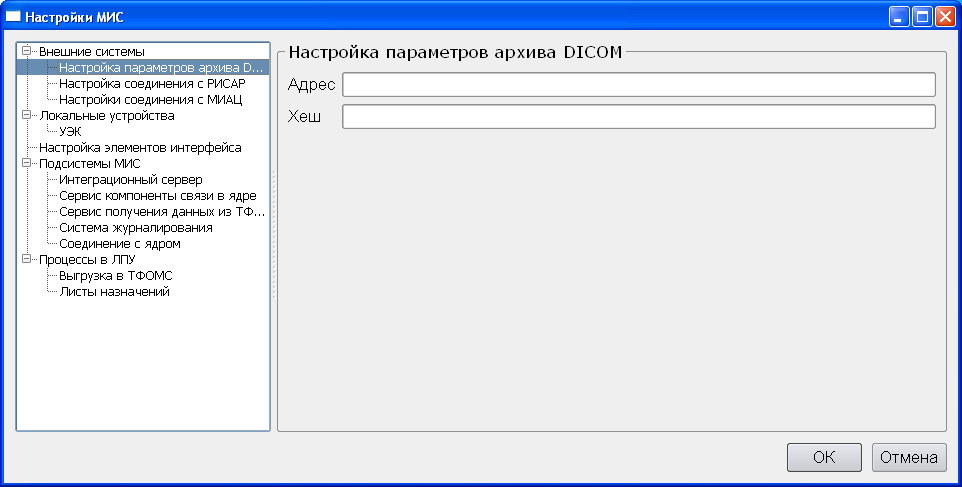
\includegraphics[width = 0.8\textwidth ,keepaspectratio]{oth_dicomm}
 \caption{Настройка соединения с внешними системами}
 \label{img_oth_dicomm}
\end{figure}

Для настройки соединения с внешней системой необходимо двойным щелчком мыши выбрать название системы в разделе \dm{Внешние системы} в левой части открывшейся формы, после чего в правой части указать параметры взаимодействия с выбранной системой. После внесения всех необходимых настроек следует сохранить их, нажав кнопку \btn{OK} в правом нижнем углу формы.

\subsection{Настройка внешнего вида}

В \tmis~могут быть изменены названия некоторых полей, что позволяет использовать систему за пределами РФ.

Для изменения названий полей следует выбрать пункт меню \mm{Настройки \str Настройки \tmis} и в левой части открывшейся формы дважды щелкнуть по наименованию \dm{Настройка элементов интерфейса}. В правой части формы (Рисунок \ref{img_oth_interf}) появятся следующие настройки:
\begin{itemize}
 \item \dm{Уникальный идентификатор гражданина} -- выбирается из раскрывающегося списка наименование уникального идентификатора гражданина, которое в дальнейшем будет использоваться на формах. Для РФ таким идентификатором является СНИЛС.
 \item \dm{Изменить наименование <<КЛАДР>> на} -- после ввода текста в данное поле, во всех формах наименование <<КЛАДР>> классификатора адресов будет заменено на указанное.
 \item \dm{Изменить наименование <<ОГРН>> на} -- после ввода текста в данное поле, во всех формах наименование <<ОГРН>> организации будет заменено на указанное.
 \item \dm{Изменить наименование <<ИНН>> на} -- после ввода текста в данное поле, во всех формах наименование <<ИНН>> организации будет заменено на указанное.
 \item \dm{Скрывать реквизиты <<КПП>>, <<ФСС>>, <<ОКВЭД>>, <<ОКАТО>>, <<ОКПФ>>, <<ОКФС>>, <<ИНФИС>>, <<Устаревший ИНФИС>>, <<Код МИАЦ>>} -- при установке данного флажка указанные поля будут скрыты в справочнике и карточках организаций.
 \item \dm{Скрывать область ввода данных по полису ОМС} -- при установке данного флажка будет скрыт подраздел ввода данных полиса ОМС в регистрационной карточке пациента.
 \item \dm{Скрывать область ввода данных по полису ДМС} -- при установке данного флажка будет скрыт подраздел ввода данных полиса ДМС в регистрационной карточке пациента.
 \item \dm{Документ, удостоверяющий личность, необходим для соц.статусов} -- при установке данного флажка становится обязательным указание документа, подтверждающего соц.статус, в регистрационной карточке пациента.
\end{itemize} 

\begin{figure}[ht]\centering
 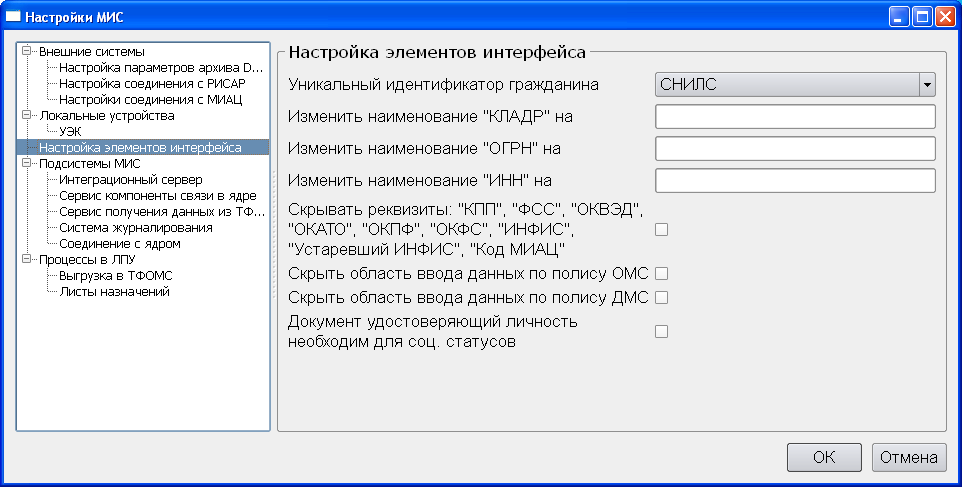
\includegraphics[width = 0.8\textwidth ,keepaspectratio]{oth_interf}
 \caption{Настройка элементов интерфейса}
 \label{img_oth_interf}
\end{figure}

После внесения всех необходимых настроек следует сохранить их, нажав кнопку \btn{OK} в правом нижнем углу формы.

\subsection{Система журналирования}

Система журналирования – это внешний модуль, подключение которого позволяет вести лог следующих действий в \tmis:
\begin{itemize}
 \item Авторизация пользователя в системе;
 \item Печать документа;
 \item Тип действия: создание, удаление, изменение;
 \item Событие: создание, удаление, изменение;
 \item Действие: создание, удаление, изменение;
 \item Ошибки, связанные с ошибками работы, обращениями в БД.
\end{itemize}
 
Для включения или отключения системы журналирования в \tmis~следует выбрать пункт \mm{Настройки \str Настройки \tmis}. В открывшейся форме слева, в группе <<Подсистемы \tmis>>, нужно выбрать пункт \dm{Система журналирования} двойным щелчком левой кнопки мыши (Рисунок \ref{img_oth_jur}).

\begin{figure}[ht]\centering
 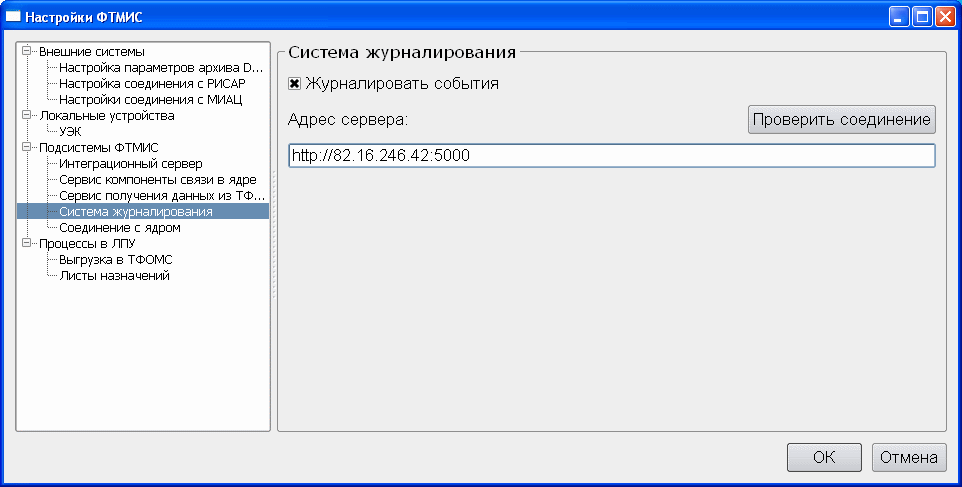
\includegraphics[width = 0.8\textwidth ,keepaspectratio]{oth_jur}
 \caption{Настройка системы журналирования}
 \label{img_oth_jur}
\end{figure}

Для ведения лога перечисленных выше событий необходимо установить флаг \dm{Журналировать события} и в строке \dm{Адрес сервера} указать адрес и порт сервера, по которым доступна система журналирования. После указания адреса рекомендуется выполнить проверку наличия соединения с системой журналирования, нажав кнопку \btn{Проверить соединение} . В случае успешного соединения, на экране появится сообщение (Рисунок \ref{img_oth_jur_con}). В случае получения сообщения об ошибке соединения, следует исправить адрес и выполнить проверку снова.

\begin{figure}[ht]\centering
 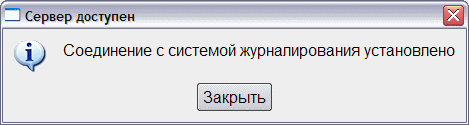
\includegraphics[width = 0.5\textwidth ,keepaspectratio]{oth_jur_con}
 \caption{Сообщение об успешном соединении с сервером журналирования}
 \label{img_oth_jur_con}
\end{figure}

\begin{vnim}
Сохранение флага включения системы журналирования возможно только после выполнения проверки соединения с сервером
\end{vnim}

Для того чтобы настройки вступили в силу, нужно сохранить их, нажав кнопку  \btn{OK} в правом нижнем углу формы.

Для отключения ведения лога событий следует снять флаг \dm{Журналировать события} и нажать кнопку \btn{OK} в правом нижнем углу формы.

\subsection{Листы назначений} \index{Листы назначений (настройки)}

Для доступа к настройкам листов назначений необходимо в главном меню выбрать пункт \mm{Настройки \str Настройки \tmis}. В открывшемся окне слева, в группе <<Процессы в ЛПУ>>, выбрать пункт \dm{Листы назначений} двойным щелчком левой кнопки мыши. При этом в правой части окна появятся настройки (Рисунок \ref{img_oth_ln}).

\begin{figure}[ht]\centering
 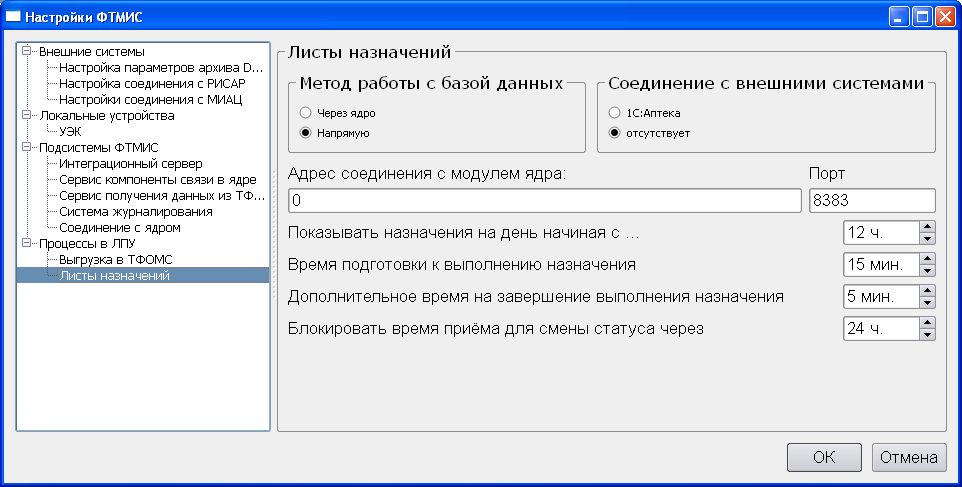
\includegraphics[width = 0.8\textwidth ,keepaspectratio]{oth_ln}
 \caption{Настройка листов назначений}
 \label{img_oth_ln}
\end{figure}

Для организации работы с листами назначений имеются следующие настройки:
\begin{itemize}
 \item \dm{Метод работы с базой данных} определяет способ взаимодействия с ядром. Следует всегда выбирать значение <<Напрямую>>.
 \item \dm{Соединение с внешними системами}: на текущий момент поддерживается только взаимодействие с системой <<1С:Аптека>>. Если в данном пункте выбрано значение <<1С: Аптека>>, то
 \begin{itemize}
  \item движение пациентов в стационаре будет передаваться в <<1С:Аптека>>;
  \item из <<1С:Аптека>> будет запрошен справочник медикаментов (РЛС);
  \item при поиске препаратов для добавления в лист назначений пациента будет производиться запрос остатков по препаратам найденной группы в <<1С:Аптека>>;
  \item будет выполняться полное обновление остатков по препаратам 1 раз в сутки (в 1:30).
 \end{itemize} 
 \item \dm{Адрес соединения с модулем ядра} необходимо указать, только в случае, если осуществляется взаимодействие с <<1С:Аптека>>. В данной строке указывается IP-адрес сервера размещения ядра.
 \item \dm{Порт} соединения с модулем ядра необходим только в случае, если осуществляется взаимодействие с <<1С:Аптека>>.
 \item \dm{Показывать назначения на день начиная с} определяет час суток, начиная с которого выполняется графление суточного листа назначений в системе Рекомендуемое значение – 12 часов.
 \item \dm{Время подготовки к выполнению назначения} определяет за сколько минут до наступления времени приема препарата оно переходит в состояние «Выполняется» (время на приготовление препарата). Рекомендуемое значение – 15 минут.
 \item \dm{Дополнительное время на завершение выполнения назначения} определяет количество минут, на сколько задерживается переход из состояния «Выполняется» после завершения интервала приема препарата. Рекомендуемое значение – 5 минут.
 \item \dm{Блокировать время приема для смены статуса через} определяет время, в течении которого можно поставить отметку о выполнении либо отменить назначение, после завершения времени приема препарата. По истечении указанного времени от момента окончания назначенного времени приема препарата, он становится недоступным для редактирования. Рекомендуемое значение – 24 часа.
\end{itemize} 

\subsection{Настройки для выгрузки в ТФОМС}

Для настройки обязательности некоторых полей, необходимых для выгрузки в ТФОМС необходимо выбрать пункт \mm{Настройки \str Настройки \tmis}. В открывшейся форме слева, в группе <<Процессы в ЛПУ>>, нужно выбрать пункт \dm{Выгрузка в ТФОМС} двойным щелчком левой кнопки мыши (Рисунок \ref{img_oth_tfoms}).

\begin{figure}[ht]\centering
 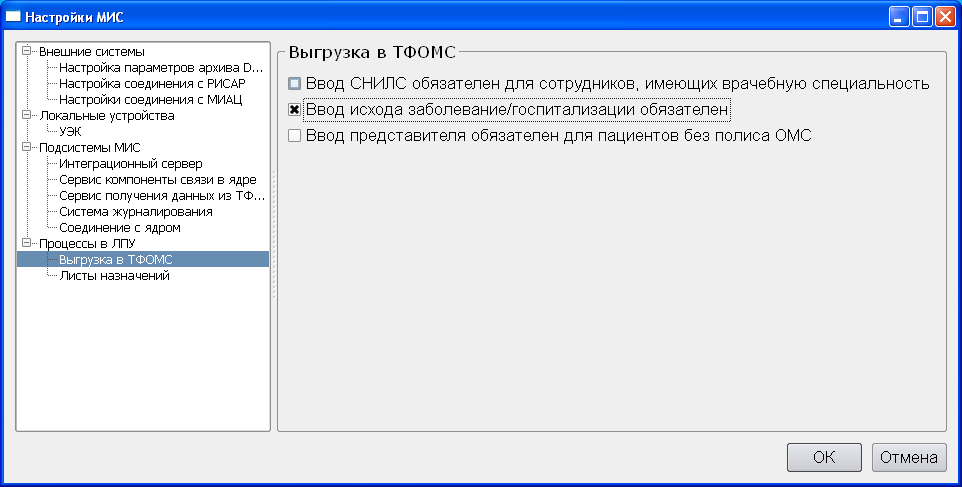
\includegraphics[width = 0.8\textwidth ,keepaspectratio]{oth_tfoms}
 \caption{Настройка обязательности некоторых полей}
 \label{img_oth_tfoms}
\end{figure}

В данном разделе можно настроить обязательность заполнения следующих полей:
\begin{itemize}
 \item \dm{Ввод СНИЛС обязателен для сотрудников, имеющих врачебную специальность} -- настройка обязательности заполнения поля СНИЛС для врачей в справочнике сотрудников (\mm{Справочники \str Персонал \str Сотрудники});
 \item \dm{Ввод исхода заболевания\slash госпитализации обязателен} -- настройка обязательности заполнения поля \dm{Исход}  в карточке обращения;
 \item \dm{Ввод представителя обязателен для пациентов без полиса ОМС} -- при установке данного флажка становится обязательным добавление представителя на вкладку \dm{Связи} регистрационной карточки пациента в случае, если не введены данные полиса ОМС данного пациента.
\end{itemize}

Для того чтобы настройки вступили в силу, нужно сохранить их, нажав кнопку  \btn{OK} в правом нижнем углу формы. 

\subsection{Настройка счетчиков}

Для многих событий, регистрируемых в \tmis, требуется вести отдельную нумерацию. Например, должен вестись отдельный учет поликлинических и стационарных обращений. Формат номеров обращений и механизм учета (в частности, номеров историй болезни) утвержден и используется уже очень давно. Чтобы не ломать привычный механизм работы в ЛПУ, \tmis~позволяет вести нумерацию событий с помощью гибко настраиваемого механизма счетчиков.

Порядок работы со счетчиками следующий:
\begin{enumerate}
 \item В пункте меню \mm{Настройки \str Счетчики} регистрируется и настраивается новый счетчик (см. ниже).
 \item В справочнике \dm{Типов событий} (\mm{Справочники \str Учет \str Типы событий}) организуется связь с данным счетчиком. Для этого на вкладке \dm{Основная информация} следует установить флажок \dm{Требуется ввод внешнего идентификатора} и в поле \dm{Счетчик} выбрать созданный в п. 1 тип счетчика.
\end{enumerate}

После выполнения указанных настроек всем событиям данного типа будут присваиваться внешние идентификаторы в соответствии с настройками нового счетчика.

\begin{figure}[ht]\centering
 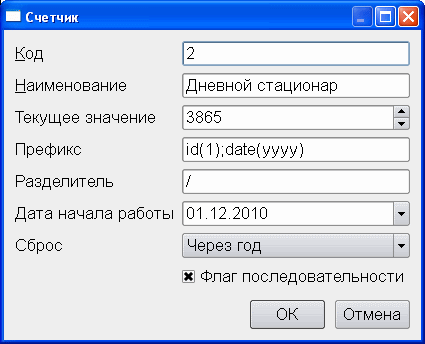
\includegraphics[width = 0.5\textwidth ,keepaspectratio]{oth_cnt}
 \caption{Карточка редактирования счетчика}
 \label{img_oth_cnt}
\end{figure}

При создании счетчика в пункте меню \mm{Настройки \str Счетчики} необходимо выполнить следующие настройки (Рисунок \ref{img_oth_cnt}):
\begin{itemize}
 \item \dm{Код} – уникальный код счетчика;
 \item \dm{Наименование} – наименование счетчика, отражающее его назначение;
 \item \dm{Текущее значение} – при создании счетчика следует указать начальное значение создаваемого счетчика. В дальнейшем, при создании событий, связанных с данным счетчиком, значение поля будет меняться автоматически. Изменять его вручную не рекомендуется.
 \item \dm{Префикс} – Номер события может быть составным. В начале указывается некоторый префикс, например, номер года для историй болезни, а затем, через разделитель, собственно номер события. Префикс может содержать несколько значений. В этом случае все они будут отображаться через разделитель. Пустые префиксы не отображаются. Например, если в поле префикс указано <<id(1);date(yyyy)>>, то номер события будет иметь формат <идентификатор пациента>/<номер года>/<текущее значение счетчика>, где <идентификатор пациента> – это идентификатор пациента во внешней системе с кодом <<1>> (раздел \ref{oth_outsys}). Если данный идентификатор у пациента отсутствует, то номер события будет иметь формат <номер года>/<текущее значение счетчика>.
 \item \dm{Разделитель} – символ разделителя, устанавливаемый между префиксом и основным номером;
 \item \dm{Дата начала работы} – устанавливается автоматически при создании счетчика;
 \item \dm{Сброс} – периодичность обнуления счетчика. Например, нумерация историй болезни пациентов начинается заново каждый год, поэтому для событий данного типа следует устанавливать значение поля \dm{Сброс} = <<Через год>>;
 \item При установке флажка \dm{Флаг последовательности} будут использоваться последовательные уникальные номера.
\end{itemize}

\subsection{Настройка выходных и праздничных дней}

При работе \tmis~используется стандартный календарь. Выходными днями считаются суббота и воскресенье. Национальные праздники не учитываются в стандартном календаре. Однако, в системе существует возможность настройки праздничных дней и переносов выходных дней. При добавлении праздничного дня или переноса выходного дня он будет отображаться красным цветом в календаре, но при составлении расписания такие выходные дни не учитываются.

Для выполнения настроек выходных и праздничных дней следует выбрать пункт меню \mm{Настройки \str Календарь}. В открывшемся окне (Рисунок \ref{img_oth_hol}) на вкладке \dm{Праздники} следует ввести все праздничные дни в году. Праздники будут автоматически распространяться на все последующие годы. Если какой-либо праздник вводится вновь или отменяется, рекомендуется использовать поля указания года начала и\slash или окончания праздника совместно с флажками \dm{Есть год начала} и\slash или \dm{Есть год окончания} соответственно.
 
\begin{figure}[ht]\centering
 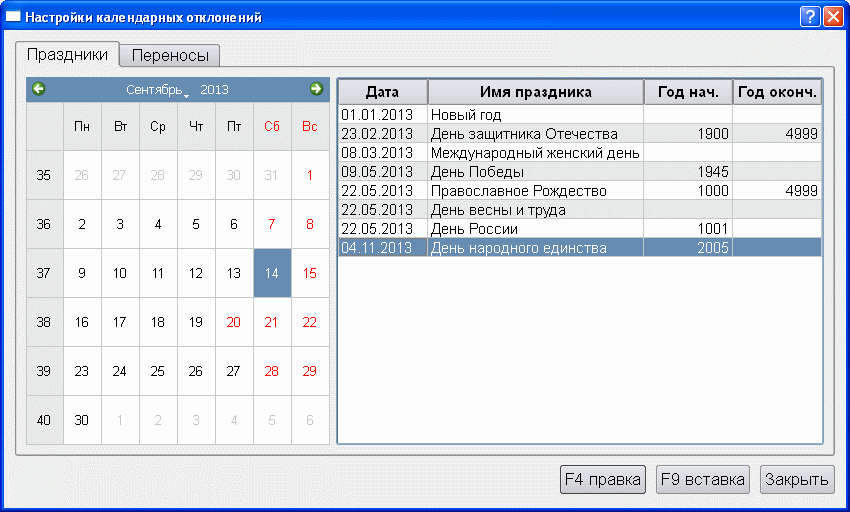
\includegraphics[width = 0.6\textwidth ,keepaspectratio]{oth_hol}
 \caption{Настройка праздничных дней}
 \label{img_oth_hol}
\end{figure}

На вкладке \dm{Переносы} можно настроить переносы выходных дней в связи с тем, что праздники выпадают на выходные. Настройка относится только к определенной дате указанного года и не распространяется на последующие годы. В поле \dm{Дата} (Рисунок \ref{img_oth_hol_per}) следует указать дату, которая становится выходным днем в связи с переносом, в поле \dm{Дата переноса} ввести исходную праздничную дату, которая выпала на выходной.

\begin{figure}[ht]\centering
 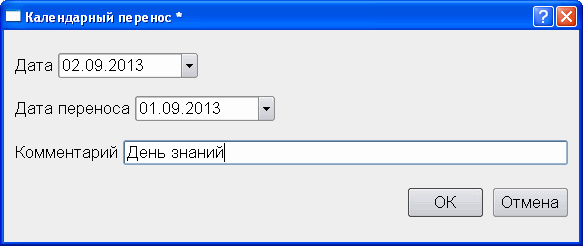
\includegraphics[width = 0.6\textwidth ,keepaspectratio]{oth_hol_per}
 \caption{Настройка переносов выходных дней}
 \label{img_oth_hol_per}
\end{figure}

\subsection{Создание правил для записи на прием}

В \tmis~возможно организовать квотирование записи пациентов на прием по времени или количеству пациентов. Настройки квотирования по времени выполняются в окне редактирования расписания сотрудника (\mm{Работа \str Учет рабочего времени}). Настройка квотирования по количеству пациентов выполняется в карточке сотрудника (\mm{Справочники \str Персонал \str Сотрудники}). При использовании метода квотирования по времени, в случае если часть талонов по какой-либо квоте остается неиспользованной, можно настроить автоматический переход неиспользованных талонов в другой тип за день или в день приема.

Настройка производится в пункте меню \mm{Настройки \str Правила записи на прием} (Рисунок \ref{img_oth_rule_per}). Редактирование и добавление записей нужно производить прямо в таблицу на форме, указав следующие данные:
\begin{itemize}
 \item \dm{Вид записи, из которого переходят талоны} (выбирается из списка);
 \item \dm{Вид записи, в который переходит талоны} (выбирается из списка);
 \item \dm{День перехода} (выбирается из списка). Можно выбрать значение <<За день до приема>> или <<В день приема>>;
 \item \dm{Время перехода} – время суток, в которое будет осуществлен переход. По умолчанию устанавливается время <<00:00>>;
 \item При установке флажка \dm{Талоны доступны для исходного вида записи}, будет возможна запись как по старой, так и по новой квоте. Если флажок не установлен, то после перехода будут доступны талоны только по новой квоте.
\end{itemize}

\begin{figure}[ht]\centering
 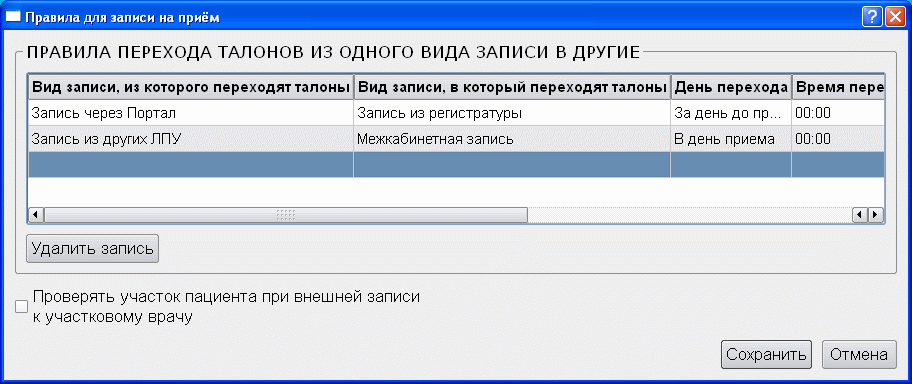
\includegraphics[width = 0.8\textwidth ,keepaspectratio]{oth_rule_per}
 \caption{Настройка правил перехода талонов}
 \label{img_oth_rule_per}
\end{figure}

\subsection{Внешние учетные системы} \label{oth_outsys}

В \tmis~существует возможность хранения идентификаторов пациентов в других информационных системах, что позволяет идентифицировать пациента и организовать получение и передачу данных пациентов в различные системы. Ввод и редактирование идентификаторов пациента во внешних системах производится в карточке пациента на вкладке \dm{Идентификаторы}.

Типы внешних систем, идентификаторы которых могут храниться в карточке пользователя, настраиваются в пункте меню \mm{Настройки \str Внешние учетные системы} (Рисунок \ref{img_oth_outsys}). Для пациента может быть сохранен только один идентификатор каждого типа, но количество типов идентификаторов при этом не ограничено и определяется только настройками справочника.

\begin{figure}[ht]\centering
 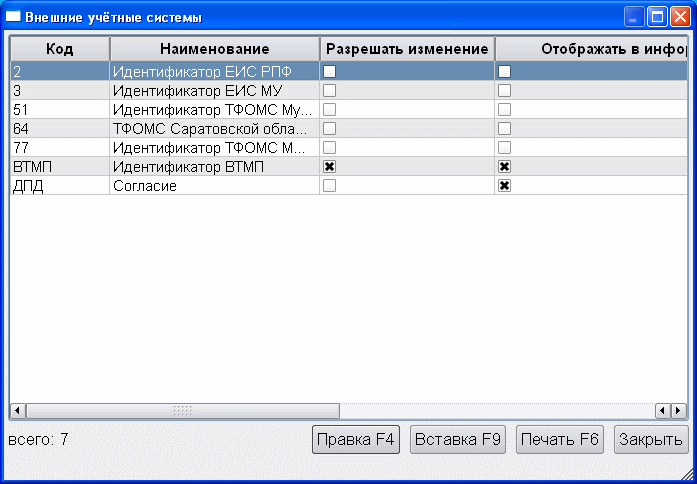
\includegraphics[width = 0.8\textwidth ,keepaspectratio]{oth_outsys}
 \caption{Справочник внешних учетных систем}
 \label{img_oth_outsys}
\end{figure}

\dm{Код} типа идентификатора должен быть уникальным, в поле \dm{Наименование} вводится название идентификатора, которое будет отображаться в карточках пациентов и фильтрах системы. Если флаг \dm{Разрешить изменение} не установлен, то редактирование ранее введенных идентификаторов невозможно.

\subsection{Настройка обмена с ТФОМС}

Настройки форматов обмена с ТФОМС производятся в отдельной системе~– Системе администрирования ЛПУ.

\subsection{Сообщения информатора}

В пункте меню \mm{Настройки \str Сообщения информатора} администратор системы может отправить \opr{всем} пользователям информационные сообщения. Сообщения будет выведено на экран пользователя при следующем входе в систему. Так же пользователь может просмотреть сообщения из пункта меню \mm{Сессия \str Информатор}.

\subsection{Настройки, выполняемые непосредственно В БД}

\subsubsection{Настройки, необходимые для работы листов назначений} \index{Листы назначений (настройки)}

\paragraph{Настройки складов для учета наличия медикаментов}

\begin{vnim}
 Данная настройка требуется только если организовано взаимо\-дей\-ствие с <<1С:Аптека>>
\end{vnim}
 
На данный момент настройку складов можно производить только непосредственно в таблице \code{rbStorage} базы данных. Структура таблицы приведена ниже.

\begin{table}
\small
\topcaption{Структура таблицы rbStorage} \label{tbl_oth_rbstor} 
 \begin{tabular}{|p{4cm}|p{4cm}|p{8.7cm}|}
  \hline \rule{0pt}{15pt} \centering \textbf{Поле} & \centering \textbf{Тип данных} & \hfil \textbf{Краткое описание} \\ \hline
  id &	INT &	Идентификатор  \\ \hline
  uuid &	VARCHAR(50) &	UUID \\ \hline 
  name &	VARCHAR(256) &	количество препарата в его единицах измерения (rlsNomen.unit\_id)  \\ \hline
  orgStructure\_id &	INT &	ссылка на отделение (OrgStructure.id)  \\ \hline  
 \end{tabular}
\end{table}

Информация в данную таблицу заносится автоматически при получении данных из <<1С: Аптека>>. Но может потребоваться изменение привязки склада к отделению. К одному отделению может относиться несколько складов (например, склад наркотических веществ и склад прочих медикаментов). От правильной организации связи склада и отделения зависит корректность отображения остатков в отделении для врача при выборе препарата.

Для того чтобы привязать склад к другому отделению, следует изменить поле \code{orgStructure\_id} , указав в нем id отделения, к которому должен быть привязан склад. Другие поля таблицы изменять не нужно!

\paragraph{Настройка источников финансирования}  

\begin{vnim}
Данная настройка требуется только если организовано взаимодействие с <<1С:Аптека>>
\end{vnim}

Для корректной выдачи и списания препаратов по источникам финансирования необходимо заполнить таблицу БД \code{rbFinance1C} соответствия кодов источников финансирования, принятых в МИС и в 1С. Таблица имеет следующую структуру:

\begin{table}
\small
\topcaption{Структура таблицы rbFinance1C} \label{tbl_oth_rbfin1c} 
 \begin{tabular}{|p{4cm}|p{4cm}|p{8.7cm}|}
  \hline \rule{0pt}{15pt} \centering \textbf{Поле} & \centering \textbf{Тип данных} & \hfil \textbf{Краткое описание} \\ \hline
  id &	INT &	Идентификатор  \\ \hline
  code1C	& VARCHAR(50) &	Код в 1С \\ \hline
  finance\_id	& INT	& Код соответствующего источника финансирования в \tmis~ {rbFinance.id} \\ \hline
 \end{tabular}
\end{table}

\begin{vnim}
 В качестве кодов <<1С:Аптека>> используются не числовые, а символьные коды. Например, <<ОМС>>, <<Платные услуги>> и т.п.
\end{vnim} 